\documentclass[twocolumn,11pt]{article}
\usepackage[T1]{fontenc}
\usepackage[utf8]{inputenc}
\usepackage{lmodern}
\usepackage{graphicx}
\graphicspath{ {images/} }

\title{Estação Meteorológica IoT}
\author{Koscianski Vidal, Davi \and Citti, Eduardo}

\begin{document}

\maketitle

\tableofcontents

\begin{abstract}
A previsão do tempo e caracterização do clima podem ser utilizadas em diversas aplicações, por exemplo automação residencial. Uma estação meteorológica utilizando conceitos de IoT (\textit{Internet of Things}) pode ser, portanto, um primeiro passo para a confecção de uma estação de automação residencial.
Utilizando sensores de umidade, temperatura, velocidade do vento e pressão atmosférica, um microcontrolador e um protocolo de comunicação, pudemos desenvolver uma estação meteorológica portátil com conexão à internet, para publicação das medidas e posterior utilização.
\end{abstract}
\section{Introdução}
Uma estação meteorológica pode ser definida com:
“(...) um local onde são recolhidos dados para análise do tempo meteorológico. Encontram-se equipadas com instrumentos (ou sensores eletrônicos) de medição e registro das variáveis meteorológicas / climáticas. Os seus dados são utilizados para a previsão do tempo e para a caracterização do clima, pelo que também podem ser designadas por estações climatológicas. Em nossos dias, por meio de programas de computador, integram-se os dados coletados, permitindo a sua apresentação. Na maior parte das estações de última geração os dados são enviados para computadores remotos, através de linhas telefónicas, rede GSM ou outros meios de transmissão.” \cite{wikiestacao}
O objetivo deste trabalho foi desenvolver uma estação meteorológica com conceitos de IoT ({\textit{Internet of Things}). Para tanto, a estação precisou ser pequena e portátil, bem como possuir algum tipo de conexão com a internet. Os sensores escolhidos foram barômetro, termômetro, anemômetro e higrômetro.
\section{Desenvolvimento}
Considerando o objetivo deste trabalho, escolhemos priorizar os sensores e seus funcionamentos, tendo quaisquer funciconalidades alheias a isso como secundárias, tais como:
\begin{itemize}
\item conexão com a internet
\item consumo de energia
\item segurança de dados
\item autonomia
\item inteligência
\item tolerância à falhas
\end{itemize}
Essa foi, portanto, a justificativa para os equipamentos e componentes utilizados neste trabalho.\par
O desenvolvimento foi inteiramente modular, tratando cada sensor como se fosse um software à parte. Isso facilitou o desenvolvimento do software, bem como o desenvolvimento do hardware e solução de eventuais problemas normais no decorrer do projeto.\par
O software foi desenvolvido utilizando a linguagem C, por se tratar de uma linguagem prática, concisa e com vasta informação para eventuais consultas.\par
\subsection{Equipamentos}
\begin{itemize}
\item Computador com sistema Linux e ambiente de desenvolvimento
\item Fonte de alimentação
\item Tacômetro
\item Ventilador
\item Protoboard
\item Multímetro
\item Raspberry Pi 3B
\item 1 Cartão de memória 16GB classe 10
\item 1 Case de acrílico
\end{itemize}
\subsection{Componentes}
\begin{itemize}
\item 1 Sensor DS18B22
\item 1 Sensor DHT22
\item 1 Chave óptica PHCT203
\item 1 Barômetro BMP180
\item 4 Resistores (\(3 \times 10 k\Omega, 220 \Omega\))
\item 1 Bateria tipo power bank
\end{itemize}

\subsection{Barômetro}
O barômetro é um instrumento científico utilizado em meteorologia para medir a pressão atmosférica. Através da pressão atmosférica, podemos saber diversas informações, entre elas, a tendência do tempo, ou seja, uma pequena previsão do tempo informando se teremos chuva, ou sol, dentro de um curto espaço de tempo. Altas pressões resultam na descida do ar frio, e baixas pressões podem produzir chuva, neve ou tempestade.\par

P=P0  e-Mg(z-z0)RT    (P0 é a pressão na altitude z0)

hPa (Hectopascal)

\subsection{Termômetro}
O termômetro é um aparelho usado para medir a temperatura ou as variações de temperatura. É um instrumento composto por um elemento sensor que possua uma propriedade termométrica, isto é, uma propriedade que varia com a temperatura. O termômetro é um sensor de temperatura.\par
Dentro do formalismo da termodinâmica, que leva em conta apenas grandezas macroscopicamente mensuráveis, a temperatura é, de forma equivalente, definida como a derivada parcial da energia interna U em relação à entropia S para um sistema em equilíbrio termodinâminco:\par

\subsection{Anemômetro}
Anemômetro é um instrumento utilizado para medir a velocidade de um fluido, como por exemplo ar ou água. Também pode ser utilizado em modelos físicos em laboratórios de hidráulica, de aerodinâmica ou, ainda, em qualquer outro fluido como os gases existentes em estrelas e planetas.
\subsection{Higrômetro}
Um higrômetro é um instrumento que serve para medir a umidade presente nos gases, mais especificamente na atmosfera. É utilizado principalmente em estudos do clima, mas também em locais fechados onde a presença de umidade excessiva ou abaixo do normal poderia causar danos, por exemplo, em peças de museus, documentos de bibliotecas e elementos de laboratórios.\par
UR= eaeS 

\subsection{Software}
\subsubsection{Protocolo}
Um dos protocolos de troca de mensagens para IoT em uso recente é o MQTT(Message Queue Telemetry Transport). Criado pela IBM no final da década de 90, obviamente o protocolo carrega muito do cenário de uso original, mais voltado e adaptado para sistemas de supervisão e coleta de dados do tipo SCADA (Supervisory Control and Data Acquisition ou Sistemas de Supervisão e Aquisição de Dados). Mas, mesmo assim, o MQTT encontrou seu espaço nesse amplo mercado de IoT.\par
O padrão de troca de mensagens no MQTT é o publish / subscriber (publicador / subscritor). Neste padrão, quando um elemento da rede deseja receber uma determinada informação, ele a subscreve, fazendo uma requisição para um outro elemento da rede capaz de gerir as publicações e subscrições. Na rede MQTT este elemento é conhecido como broker, o intermediário no processo de comunicação. Elementos que desejam publicar informações o fazem também através do broker, enviando-lhe as informações que possuem. Esse padrão não é novo e existe em outros protocolos. Por exemplo, a troca de informação de controle (links) em redes Foundation Fieldbus segue o paradigma publish / subscriber.\par
A identificação das mensagens no MQTT se dá através de tópicos (topics). O tópico lembra o conceito de URI, com níveis separados por barras ("/"). Elementos da rede podem enviar diversos tópicos para o broker e subscritores podem escolher os tópicos que desejam subscrever.\par
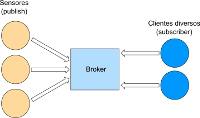
\includegraphics{mqtt_small.png}
\section{Conclusão}
A confecção modular do sistema facilitou os ensaios e as conclusões de cada etapa. Assim que cada módulo estava funcionando, conectar ao todo era um passo muito trivial, o que permitiu concluir o projeto antes do prazo de entrega.\par
O sensor DHT22, mostrou-se instável em alguns momentos, chegando até a parar de funcionar. Foi quando uma pesquisa ao datasheet trouxe a informação que este sensor pode ficar inoperante por até 5 horas, se exposto a grandes variações de temperatura, exatamente o que aconteceu em um dos testes, quando expusemos todo o sistema à um ventilador para calibração do anemômetro.\par
Na proposta do trabalho não foi mencionado a medição de pressão atmosférica, como desafio, foi adicionado um barômetro, complementando a estação IoT com mais essa aquisição de pressão, que é de extrema importância em um sistema meteorológico.

\begin{thebibliography}{9}
\bibitem{wikiestacao}
Wikipedia.
Estação Meteorológica;
Disponível em: https://pt.wikipedia.org/wiki/Esta%C3%A7%C3%A3o_meteorol%C3%B3gica .
Acesso em 16/11/2017.
\end{thebibliography}
\end{document}
